In the following part the quantities and tools used for contact analysis are briefly introduced.\\
\\
Intramolecular distances have been analysed with \conan{}. This analysis tool measures inter-residue distances and performs statistical analysis on them. \conan{} is still under development and not published yet.\\% TODO: cite Csaba?
The contact area of the FERM-kinase interface can be determined with the solvent accessible surface area (SASA) of the domains involved:
\begin{equation}
\text{CA} = \frac{1}{2} \left(\text{SASA}_\text{FERM} + \text{SASA}_\text{kinase} - \text{SASA}_\text{FERM-kinase}\right).
\end{equation}
For the calculation of SASA values \gromacs{} sasa tool was used. The v.d.W radii were adapted to \martini{} beads.\\
\\
For an appropriate description of intermolecular interactions between FAK molecules, we defined the following terms:
\paragraph{Interaction} Proteins or part of proteins interact, if their minimal distance is smaller than a cut-off distance (here $1.5\,\si{\nano\metre}$).
\paragraph{Neighbour} Two proteins are neighbours, if they are interacting with each other. One protein can have several neighbours. For a more detailed characterisation we defined the following neighbour types:
\begin{enumerate}[label={type \theenumi:}, leftmargin=*]
	\setcounter{enumi}{0}
	\item only the FERM domain interacts with only the FERM domain of the neighbouring protein
	\item only the kinase interacts with only the kinase of the neighbouring protein
	\item only the FERM domain interacts with only the kinase of the neighbouring protein
	\item the FERM domain is interacting with both, the FERM and kinase of the neighbouring protein
	\item the kinase is interacting with both, the FERM and kinase of the neighbouring protein
	\item the FERM domain is interacting with the FERM domain of the neighbouring protein and the kinase is interacting with the kinase of the neighbouring protein
	\item the FERM domain is interacting with the kinase of the neighbouring protein and the kinase is interacting with the FERM domain of the neighbouring protein
\end{enumerate}
\paragraph{Cluster} Neighbouring proteins form a cluster. A protein belongs to a cluster, if it has at least one neighbour inside the cluster. One protein can only belong to one cluster. The clustersize is the number of proteins belonging to the cluster.
%
%
%
\begin{figure}
	\centering
	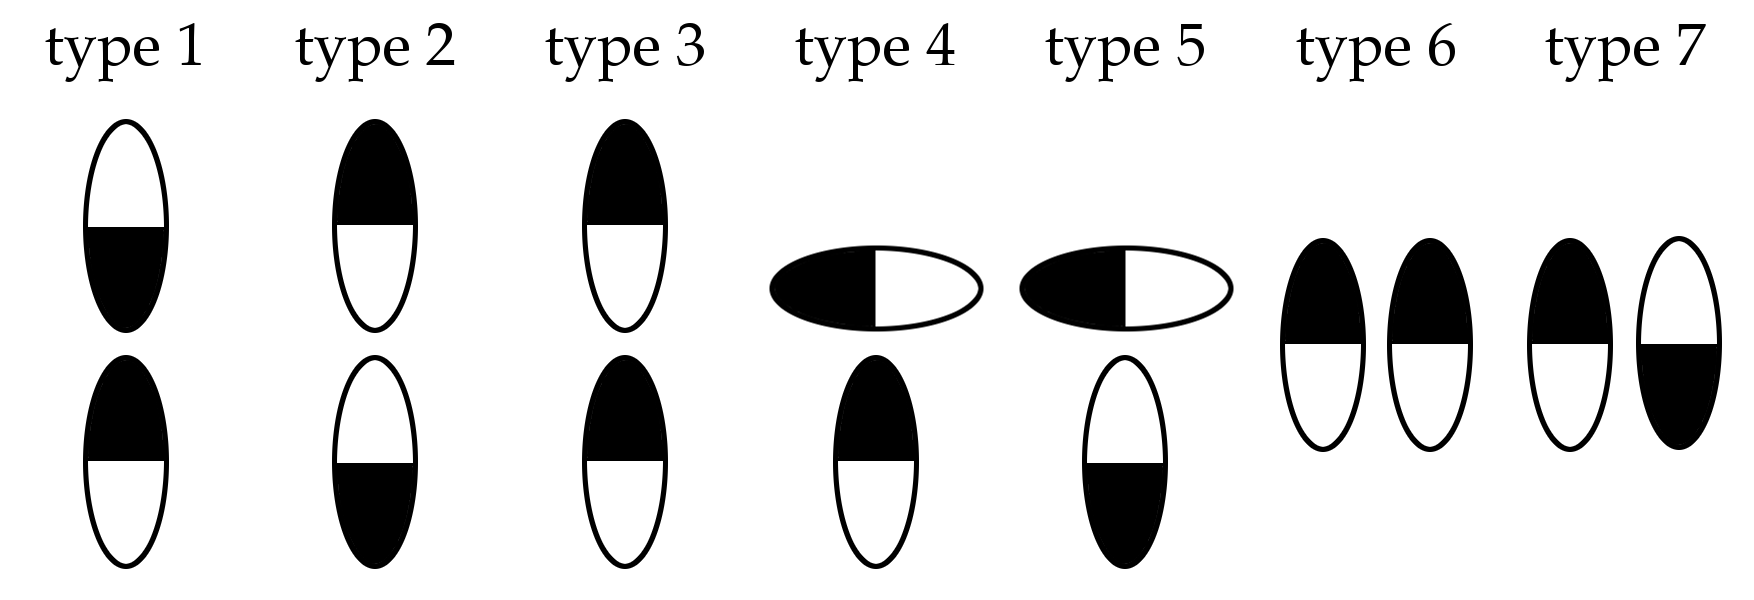
\includegraphics[width=0.6\textwidth]{figures/introduction/classification}
	\nicecaption{Different two-molecule interaction types}{The black part refers to the FERM domain, the white to the kinase.}
	\label{methods:inttypes}
\end{figure}
%
%
%